\documentclass[12pt,a4paper]{article}
\usepackage{graphicx}
\usepackage[english,ngerman]{babel}
\usepackage[parfill]{parskip} % to start each parapraph will an empty line before
\usepackage{listings}
\usepackage{hyperref}
\usepackage{float}

\begin{document}
	\begin{titlepage}
		\centering
		
\includegraphics[width=0.8\textwidth]{img/Hska_logo.png}\par\vspace{1cm}
		{\scshape\LARGE Dokumentation\par}
		\vspace{1.5cm}
		{\huge\bfseries Verteilte Systeme Master Labor\par}
		\vspace{2cm}
		{\Large\itshape Pol Zeimet (65834) \\zepo1012@hs-karlsruhe.de\par}
		\vfill
		{\Large\itshape Yannick Stephan (65934) \\stya1012@hs-karlsruhe.de\par}
		\vfill
		\large Aufgabe 1
		
		\vfill
		
		% Bottom of the page
		{\large \today\par}
	\end{titlepage}
	\section{Beschreibung}
	\label{sec:Beschreibung}
	Das zu analysierende Projekt beschreibt einen über den Browser erreichbaren Web-Shop. Der Webshop stellt mehrere Funktionen zur Verfügung, welche in diesem Abschnitt beschrieben werden.
	\begin{itemize}
	\item{Registrieren und Anmelden}\\ Beim ersten Besuch des Shops muss ein eigener Account mit Namen und Passwort erstellt werden. Bei weiteren Besuchen werden diese zum Login verwendet.
	\item{Anlegen und Löschen Kategorien}\\ Im Webshop ist es dem Nutzer möglich, Produktkategorien anzulegen und zu löschen.
	\item{Produkte erstellen und löschen}\\ Nutzer können Produkte erstellen und sie einer vorher definierten Kategorie hinzufügen. Erstellte Produkte können in der gleichen Übersicht auch gelöscht werden.
	\item{Nach Produkten suchen}\\ Produkte können nach ihren angegebenen Attributen  Preis, Name und Kategorie gefiltert und abgefragt werden.
	\end{itemize}
	\section{Aufbau}
	\subsection{MVC}
	Das Projekt ist nach dem MVC-Prinzip aufgebaut.
	\subsubsection{View}
	Die View besteht aus .jsp Dateien. Diese enthalten den Aufbau der Seite, sowie die entsprechenden auszuführenden Aktionen beim Bedienen der Schaltflächen.
	Über Struts sind die in der View beschriebenen Aktionen mit dem Controller verbunden. Bei erfolgreicher Aktion wir die in der struts.xml hinterlegte Darstellung angezeigt.
	\subsubsection{Controller}
	Der Controller besteht aus Aktionsklassen, die jeweils mit über Struts von der View aus aufgerufen werden. Die Aktionsklassen prüfen die übergebenen Parameter auf ihre Gültigkeit sowie die Berechtigungen den aktuellen Session-Kontext und somit den Nutzer und rufen dann die entsprechende Businesslogik aus dem Model auf, die zum ausführen der Aufgabe benötigt ist. Bei erfolgreicher Ausführung wird eine Bestätigung zurückgegeben.
	\subsubsection{Model}
	Das Model, also die zugrundeliegende Businesslogik, ist in den Manager-Klassen implementiert. diese Klassen enthalten die Methoden, die zum ausführen der gewünschten Nutzeraktionen benötigt werden. Dies beinhaltet Datenbankzugriffe und die Verarbeitung von Suchbegriffen.
	Die Tatsächlichen Datenbankzugriffe werden dabei nicht durch den Manager selber, sondern durch ein Data Access Objekt, kurz DAO durchgeführt.
	\subsection{Objekte}
	Der allgemeine Aufbau des Quellcodes sowie die Abhängigkeiten der verschiedenen Objekte lassen sich gut anhand eines UML Diagrammes darstellen. Der Übersicht halber werden wir uns eine einzelne Aktion ansehen, da alle Aktionen die gleiche Struktur verfolgen.\\
	So haben wir unsere Aktionsklasse, welche über eine execute() Funktion die Businesslogik des Models aufruft. Eine Aktionsklassen ist hierbei eine Erweiterte \textit{Actionsupport} Klasse, Manager Klassen implementieren ein ihrer Rolle entsprechendes Manager Interface. Da es in diesem Fall um das hinzufügen einer neuen Kategorie geht, sind die Aktions- sowie die Manager-Klasse mit der Kategorie-Klasse verknüpft. Die Validierung der Eingabe übernimmt ebenfalls die Aktionsklasse.
	Das ablegen der Kategorie in, sowie das Laden der aktualisierten Kategorie-Liste aus der Datenbank erfolgen über ein Data Access Objekt. Dieses baut auf einem HybernateDAO auf. Jedes Objekt, das in die Datenbank abgespeichert werden soll, verfügt über ein eigenes DAO. Hybernate erlaubt es uns hierbei, sogenannte "`POJOs"', "`Plain old Java objects"', also normale Java Objekte über Annotationen als Tabellen anzulegen und mit den entsprechenden Objekt-Variablen zu füllen.
	\begin{center}
%		\includegraphics[scale=0.3]{$TODO$}
	\end{center}

	
	\section{Ablauf}
	Der Ablauf der beschriebenen Funktionen aus Kapitel \ref{sec:Beschreibung} kann in  Aktivitäts-- und Klassendiagrammen zusammengefasst werden:
	
	\subsection{Registrieren und Login}
	\begin{figure}[H]
		\centering
		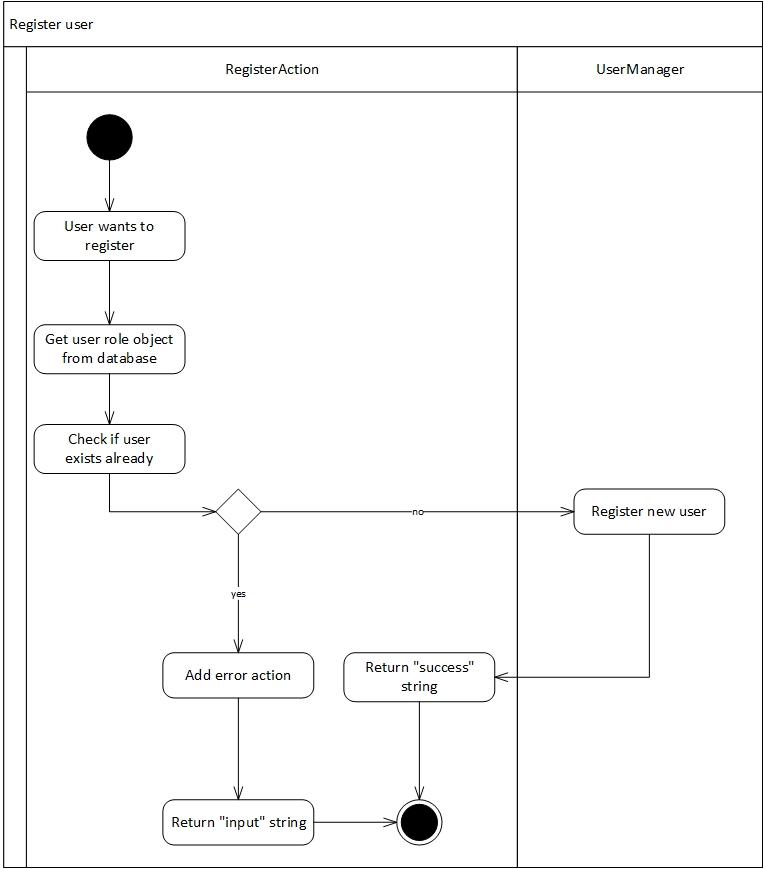
\includegraphics[scale=0.5]{diagrams/RegisterUser_activity.jpg}
		\caption{Aktivitätsdiagramm für das Registrieren eines neuen Benutzers}
	\end{figure}
	
	\subsection{Anlegen und Löschen Kategorien}
	\begin{figure}[H]
		\centering
		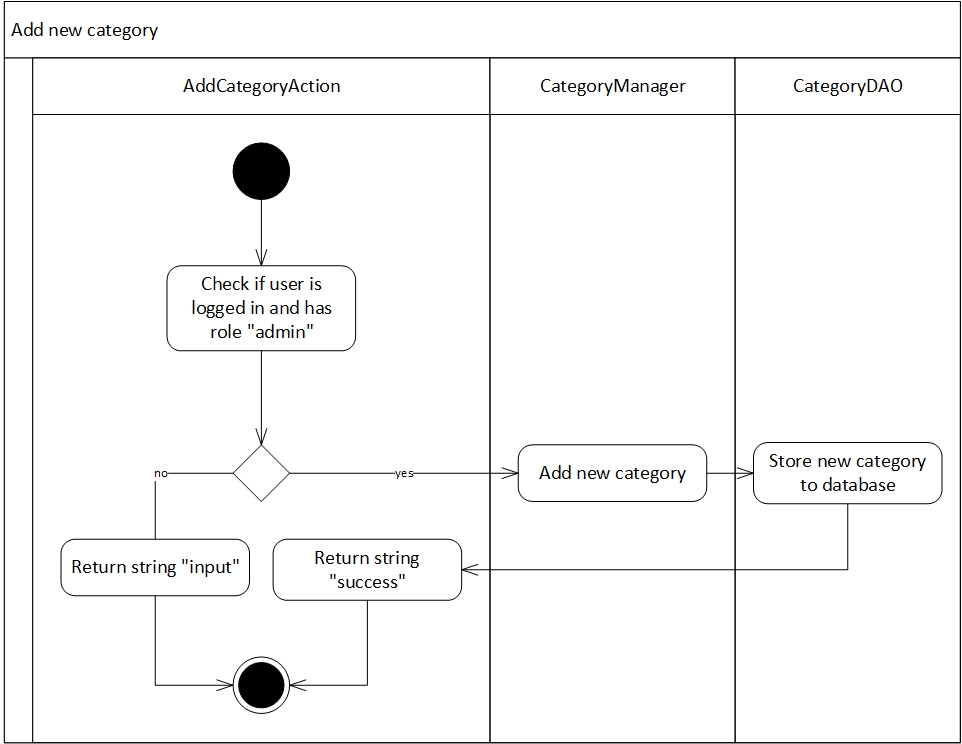
\includegraphics[scale=0.5]{diagrams/AddCategoryAction_activity.jpg}
		\caption{Aktivitätsdiagramm für das Hinzufügen neuer Kategorien}
	\end{figure}

	\begin{figure}[H]
		\centering
		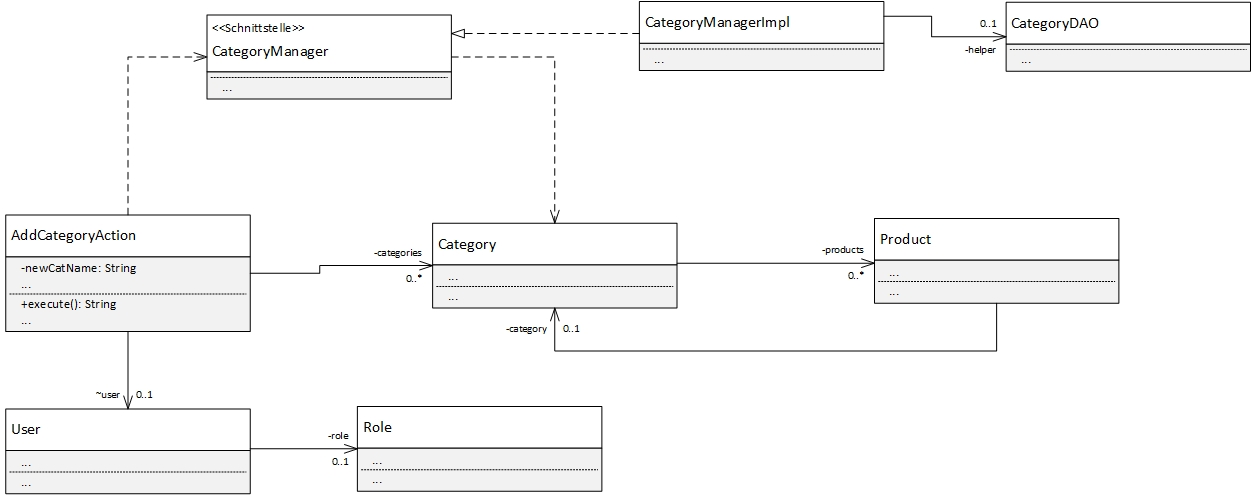
\includegraphics[scale=0.5]{diagrams/AddCategoryAction_class.jpg}
		\caption{Klassendiagramm der \textit{AddCategoryAction}}
	\end{figure}

	\begin{figure}[H]
		\centering
		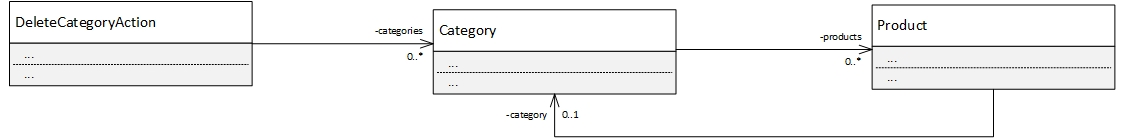
\includegraphics[scale=0.5]{diagrams/DeleteCategoryAction_class.jpg}
		\caption{Klassendiagramm der \textit{DeleteCategoryAction}}
	\end{figure}

	\subsection{Produkt erstellen und löschen}
	\begin{figure}[H]
		\centering
		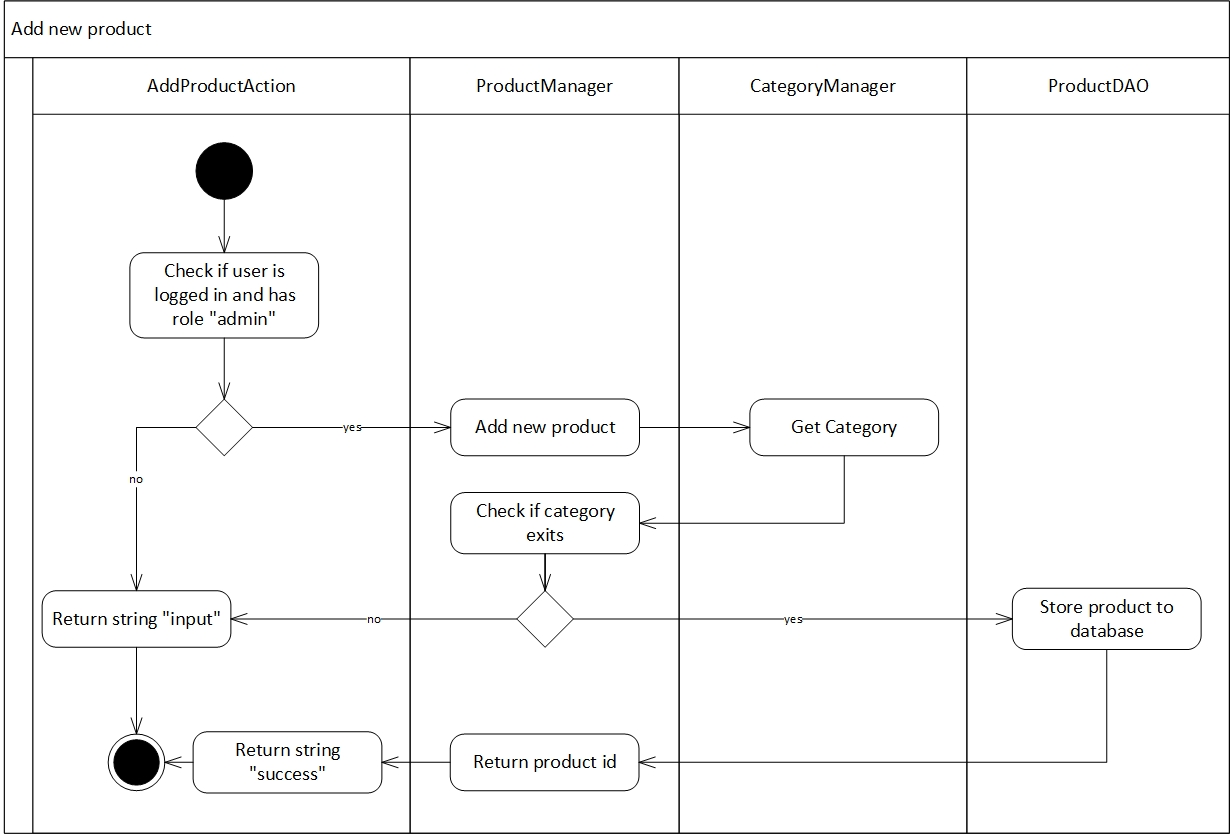
\includegraphics[scale=0.5]{diagrams/AddProductAction_activity.jpg}
		\caption{Aktivitätsdiagramm für das Hinzufügen neuer Produkte}
	\end{figure}

	\begin{figure}[H]
		\centering
		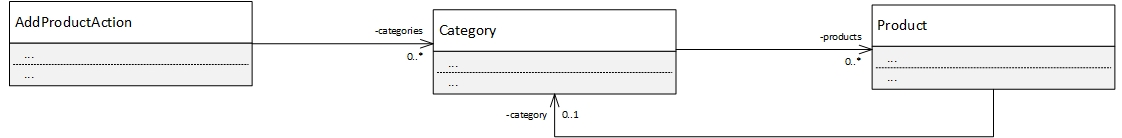
\includegraphics[scale=0.5]{diagrams/AddProductAction_class.jpg}
		\caption{Klassendiagramm der \textit{AddProductAction}}
	\end{figure}
	
	\subsection{Nach Produkten suchen}
	TODO ...
	
\end{document}